\section{Background}

This section will aim to provide a general overview of the field of evolutionary computation. General terms and procedures which are often utilized in EC will be explained and the most well known traditional approaches will be presented. The necessary concepts from machine learning will be presented.

\subsection{Evolutionary Algorithms}

Evolutionary algorithms work on the concept of populations. A population is a set of individuals which in the case of optimization problems contain a vector of parameters which the model we wish to optimize can accept and transform into an output. The population is initialized by some procedure to contain a random set of parameter vectors, these should cover the whole parameter range of the model uniformly. The initial population is evaluated and an iterative process is started which continues as long as no suitable solution is found. During this iterative process the current population is selected, altered and evaluated. During selection a set of individuals which display promising characteristics are selected to live on into the next generation of the population. They are then altered randomly to create diversity in the population and evaluated. This process creates a new generation of the population on each iteration and continues until a solution is found or some other restriction is encountered~\cite{Eiben20021}. The concept is demonstrated in figure~\ref{algo:basicevolution} with $P(t)$ representing the population at generation $t$.

\begin{algorithm}[h]

  \caption{Basic evolutionary algorithm}
  \label{algo:basicevolution}
    \begin{algorithmic}
       \State $t\gets 0$
       \State initialize $P(t)$
       \State evaluate $P(t)$
       \While{termination-condition not fulfilled}
        \State $t\gets t + 1$
        \State select $P(t)$ from $P(t-1)$
        \State alter $P(t)$
        \State evaluate $P(t)$
       \EndWhile
    \end{algorithmic}

\end{algorithm}

Here the fundamental building blocks of evolutionary algorithms will be presented and explained. Most of these term are universal to all approaches which will be covered in this thesis.

\subsubsection{Representation}

The first step in using evolutionary algorithms is creating a representation which can encode all possible solutions to the problem. Here two different terms are distinguished. The term phenotype denotes the representation that can be directly applied to the problem and the genotype denotes the specific encoding of the phenotype which is manipulated inside the evolutionary algorithm. In optimization tasks a valid phenotype could be a vector of integer numbers which act as parameters to a function while the genotype would be a binary representation of the numbers which can be altered by manipulating individuals bits. The terms phenotype, candidate solution and individual are used interchangeably to denote the representation as used by the model while chromosome, genotype and individual are used to refer to the representation inside the evolutionary algorithm~\cite{Eiben2015_whatevolutionary}.

\paragraph{Binary representation}

Genetic algorithms (GA) traditionally use a binary representation to store individual genotypes. The representations is a string of fixed length over the alphabet $\{0,1\}$. The problem thus becomes a boolean optimization problem of the form $ f:\{0,1\}^l \rightarrow \mathbb{R}$, where the mappings $h:M \rightarrow \{0,1\}^l$ and $h':\{0,1\}^l \rightarrow M$ are used to encode and decode the parameters and solutions~\cite{back1997evolutionary}. See figure~\ref{fig:bin} for an example.

\begin{figure}[H]
  \centering
  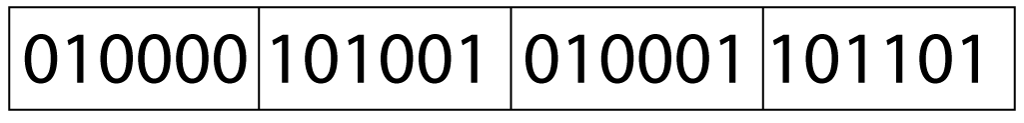
\includegraphics[width=.7\linewidth]{binary}
  \caption{Binary representation of chromosome with four genes}
  \label{fig:bin}
\end{figure}

\paragraph{Integer representation}

Integer representations have been proposed by some researches~\cite{unter611evolutionary}. This approach is useful when dealing with problems where we need to select certain elements in a particular order, e.g. graph-problems, path-finding problems, the knapsack problem, etc.~\cite{Eiben201511}. See figure~\ref{fig:int} for an example.

\begin{figure}[H]
  \centering
  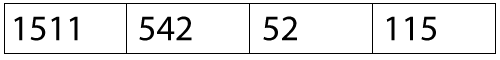
\includegraphics[width=.7\linewidth]{integer}
  \caption{Integer representation of chromosome with four genes}
  \label{fig:int}
\end{figure}


\paragraph{Real-valued representation}

Real-valued or floating-point representations were originally used in evolutionary programming and evolution strategies and work well for problems located in continuous search-spaces. The problems take the form $f:M\subseteq \mathbb{R}^n \rightarrow \mathbb{R} $~\cite{back1997evolutionary}. See figure~\ref{fig:float} for an example.

\begin{figure}[H]
  \centering
  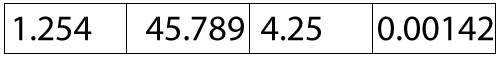
\includegraphics[width=.7\linewidth]{float}
  \caption{Real-valued representation of chromosome with four genes}
  \label{fig:float}
\end{figure}

\paragraph{Tree representation}

Tree representations are mainly used in genetic programming to capture the structure of programs. The encoding varies but S-expressions are generally used. The tree structure is defined by a function-set and a terminal-set. The function-set defines the types of nodes in the tree, while the terminal-set contains the types of leaves the tree can contain~\cite{Eiben201511}.

\subsubsection{Evaluation function}

Evaluation function is responsible for improvement in the population. It is a function which assigns a fitness or cost value to every genotype and thus enables us to compare the quality of the genotypes in the population. It is also the only information about the problem that is available to the evolutionary algorithm and should therefore include all domain knowledge which is available about the problem~\cite{Eiben2015_whatevolutionary}. The evaluation is also the process which takes up the most computational resources, 99\% of the total computational cost in real-world problems~\cite{Eiben20021}.

\subsubsection{Population}

The population is a set of genotypes which contain the current best solutions to a problem. While genotypes remain stable and unchanging, the population continually changes through the application of selection mechanisms which decide which genotypes are allowed into the next generation of the population. The size of the population almost always remains constant during the lifetime of the algorithm. This in turn creates selection pressure which pushes the population towards improvement. A population's diversity is the measure of difference among the genotypes, phenotypes and fitness values~\cite{Eiben2015_whatevolutionary}.

\paragraph{Steady-state model}

In the steady-state model the entire population isn't replaced at once. Only a fraction of the population is replaced at one time.

\paragraph{Generational model}

In the generational model the entire population is replaced at once.

\subsubsection{Parent selection mechanism}

Parent selection serves to improve the quality of a population by selecting which individuals will survive into the next generation. The selected individuals are called parents as they usually undergo some form of alteration or combination with other individuals before progressing to the next generation. The selection method is usually probabilistic and gives better solutions a higher probability and worse solutions a lower probability to survive. It's important that bad solutions still receive a positive probability since the population might otherwise lose diversity and coalesce around a false local optimum~\cite{Eiben2015_whatevolutionary}.



\paragraph{Fitness proportional selection}

Fitness proportional selection (FPS) assigns a selection probability to an individual based on it's absolute fitness. This results in very good individuals overtaking the population quickly and premature convergence. If individuals have very similar fitness values the selection pressure becomes low. This mechanism is also very dependent on the exact form of the fitness function~\cite{Eiben2015asdfasd}.

\paragraph{Ranking selection}

In ranking selection the population is sorted according to the individual's fitness values and the selection pressure is kept constant. A constant number of the best individuals is then selected from the sorted list~\cite{Eiben2015asdfasd}.

\paragraph{Tournament selection}

Tournament selection enables selection without global knowledge of the population's fitness. A number of individuals are chosen at random and the best one is selected. This process is repeated until the desired number of individuals is selected~\cite{Eiben2015asdfasd}.


\subsubsection{Variation operators}

Variation operators introduce new features into the genotypes of a population by modifying or mixing existing genotypes. They can be divided into two types: unary operators which take one genotype and stochastically alter it to introduce random change and n-ary operators which mix the features of 2 or more genotypes. Unary operators are called mutation operators while n-ary operators are called cross-over or recombination operators. The biological equivalents to these are random mutation and sexual reproduction. Mutation operators allow evolutionary algorithms to theoretically span the whole continuum of the search space by giving a non-zero probability that a genotype mutates into any other other genotype. This has been used to formally prove that evolutionary algorithms will always reach the desired optimum given enough time. Recombination tries to create new superior individuals by combining the genes of two good parent genotypes~\cite{Eiben2015_whatevolutionary, Eiben20021}.

\paragraph{Binary mutation}

The most commonly used mutation scheme for binary representations consists of randomly flipping bits (genes) in a chromosome with a certain probability. The number of alterations is not fixed with this approach, but the common procedures used can often be set to change a certain number of bits on average~\cite{Eiben201511}.

\paragraph{Binary recombination}

Three approached are normally used to recombine binary chromosomes. One-point crossover divides the chromosome into two sections, picking a random intersection point, and swaps the tails of the two chromosomes creating two offspring. N-point crossover generalizes this behavior by picking n random splitting points and assembling new chromosome by taking alternate sections of the parent chromosomes. Uniform crossover creates an array of uniform numbers from a probability distribution and chooses which parent to take a gene from by comparing the random value to a probability threshold~\cite{Eiben201511}.

\paragraph{Integer mutation}

Random resetting and creep mutation are used to mutate integer chromosomes. In random resetting integer values are changed with a certain probability. The new values are chosen at random from the pool of permissible values. Creep mutation samples small numbers from distributions and adds or subtracts them from genes at random~\cite{Eiben201511}.

\paragraph{Integer recombination}

For integer representations the same techniques that are used for binary representations apply~\cite{Eiben201511}.


\paragraph{Real-valued mutation}

For real-valued representations mutation is similar to integer mutation with the exception that new random values are drawn from continuous distributions and creep mutation uses a gaussian distribution to sample values. A lower and upper bound is used to limit the span of the generated random numbers~\cite{Eiben201511}.

\paragraph{Real-valued recombination}

There are three common ways to recombine real-valued chromosomes. Discreet recombination works like n-point crossover and thus does not alter the values in the offspring chromosomes. Arithmetic recombination chooses values which fall in-between the values of the parent chromosomes for it's offspring. Blend recombination works like arithmetic recombination but allow for values which lie slightly outside of the interval defines by the parent genes~\cite{Eiben201511}.


\paragraph{Tree mutation}

Trees are usually mutated by selecting a node at random and re-generating it's subtree using the same approach which was used to generate the initial population~\cite{Eiben201511}.

\paragraph{Tree recombination}

Subtree crossover is commonly used to recombine trees. It randomly selects a node in each tree and then swaps the respective subtrees creating two new offspring~\cite{Eiben201511}.


\subsubsection{Survivor selection mechanism}

Survivor selection takes place after new offspring have been generated and determines which individuals are allowed to live on into the next generation. It is often referred to as the replacement strategy and contrary to parent selection it is usually deterministic. Two popular mechanisms are fitness-based selection and age-based selection. Fitness-based selection determines the next generation by selecting the individuals with the highest fitness while age-based selection allows only the offspring to survive~\cite{Eiben2015_whatevolutionary}.


\subsubsection{Initatilization}

Initialization is the process during which the initial population is generated. The genotypes are usually generated randomly from a uniform distribution based on some range of acceptable input values. If a good solution is known before hand variations of it can be include in the initial population as a bias, but this can sometimes cause more problems than it solves~\cite{Eiben20021}.

\subsubsection{Termination condition}

The termination condidion determines for how long the algorithm is run. Four criteria are used to determine when to stop~\cite{Eiben2015_whatevolutionary}:

\begin{enumerate}
  \item If a maximum number CPU-cycles or iterations is reached
  \item If a known optimum is reached
  \item If the fitness value does not improve for a considerable amount of time
  \item If the diversity of the population drops below a given threshold
\end{enumerate}

\subsection{Traditional Evolutionary Algorithms}

Below the main paradigms of evolutionary computation will be discussed. They include genetic algorithms, evolution strategy, evolutionary programming and genetic programming.

\subsubsection{Genetic algorithms}

Genetic algorithms (GA) were introduced by John Holland in the 1960s as an attempt to apply biological adaptation to computational problems. GAs are multidimensional search algorithms which use populations of binary strings called chromosomes to evolve a solution to a problem. GAs use a selection operator, a mutation operator and a cross-over operator. The selection operator select individuals which are subjected to cross-over based on their fitness and cross-over combines their genetic material to form new individuals which are then randomly mutated~\cite{mitchel1999evolutionary}. See algorithm~\ref{algo:geneticalgorithm} and figure~\ref{fig:GA} for a simple GA.

\begin{figure}[H]
  \centering
  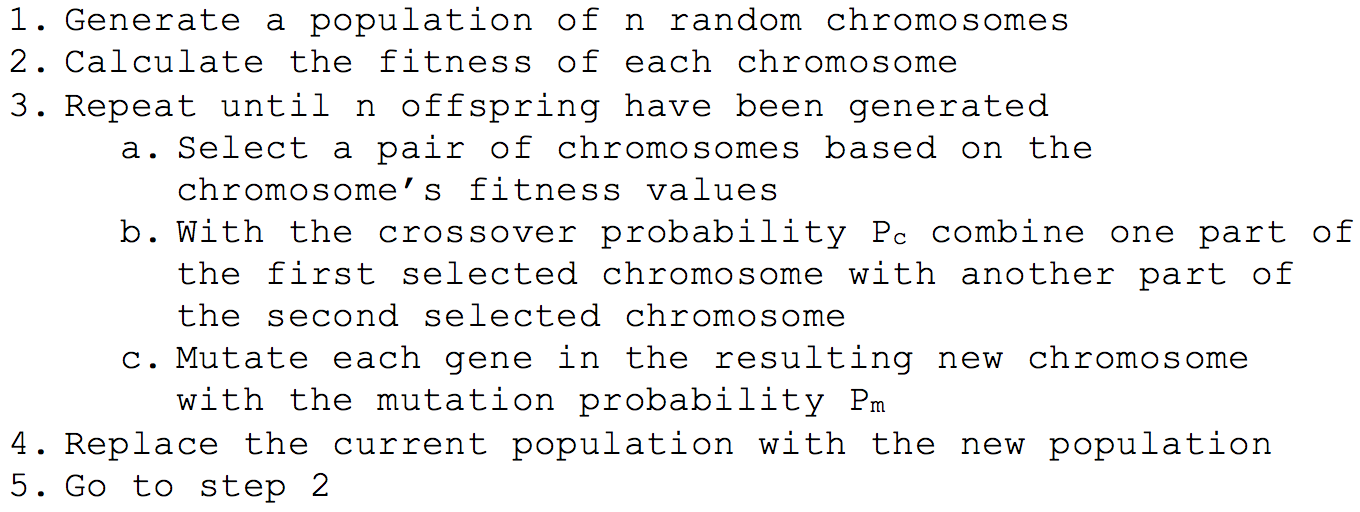
\includegraphics[width=.5\linewidth]{GA}
  \caption{Stages in GA (1) Evaluation (2) Selection (3) Crossover (4) Mutation}
  \label{fig:GA}
\end{figure}

\begin{algorithm}[h]

  \caption{Basic genetic algorithm}
  \label{algo:geneticalgorithm}
    \begin{algorithmic}
       \State Initialize a population of N binary chromosome with L bits
       \While{termination-condition not fulfilled}
        \State Evaluate the fitness $F(x)$ of each chromosome $x$
        \Repeat
          \State Select two chromosomes probabilistically from the population
          \State based on their fitness
          \State With the cross-over probability $P_c$ create two new offspring
          \State from the two selected chromosomes using the crossover operator.
          \State Otherwise create two new offspring identical to their parent chromosomes.
          \State Mutate the two chromosomes using the mutation probability $P_m$
          \State and place the resulting chromosomes into the new population
        \Until{N offspring have been created}
        \State Replace the old population with the new population
       \EndWhile
    \end{algorithmic}
\end{algorithm}

\subsubsection{Evolution strategy}

Evolution strategies (ES) were first developed to solve parameter optimization tasks. They differ from GAs by representing individuals using a pair of vectors $\vec{v} = (\vec{x},\vec{\sigma})$. The earliest versions of ES used a population of only one individual and only utilized the mutation operator. New individuals were only introduced into the population if they performed better than their parents. The vector $\vec{x}$ represents the position in the search space and $\vec{\sigma}$ represents a vector of standard deviations used to generate new individuals. Mutation occurs according to equation~\ref{eq:evolutionstrategy1} where $N(0,\vec{\sigma})$ is a vector containing random Gaussian numbers with the mean $0$ and a standard deviation of $\vec{\sigma}$~\cite{Michalewicz1997}.

\begin{equation}
  \vec{x}^{t+1} =  \vec{x}^{t} + N(0,\vec{\sigma})
  \label{eq:evolutionstrategy1}
\end{equation}

Newer versions of the algorithm include $(\mu + \lambda)-\text{ES}$ and $(\mu,\lambda)-\text{ES}$. The main point of these it that their parameters like mutation variance adapt automatically to the problem. In $(\mu + \lambda)-\text{ES}$ $\mu$ parents generate $\lambda$ offspring and the new generation is selected from $\mu$ and $\lambda$ while in $(\mu,\lambda)-\text{ES}$ $\mu$ parents generate $\lambda$ offspring ($\lambda > \mu$) and the new generation is only selected from $\lambda$. These algorithms produce offspring by first applying cross-over to combine two parent chromosomes (including their deviation vectors $\vec{\sigma}$) and then mutating $\vec{x}$ and $\vec{\sigma}$~\cite{Michalewicz1997}.

\subsubsection{Evolutionary programming}

Evolutionary programming (EP) was created as an alternative approach to artificial intelligence. The idea was to evolve finite state machines (FSM) which observe the environment and elicit appropriate responses~\cite{Fogel1996}. The environment is modeled as a sequence of input characters selected from an alphabet and the role of the FSM is to produce the next character in sequence. The fitness of an FSM is measured by a function which tests the FSM on a sequence of input characters, starting with the first character and then progressing to include one more addition character on each iteration. The function measures the correct prediction rate of the FSM and determines it's score~\cite{Michalewicz1997}.

Each FSM creates one offspring which is mutated by one or more of the following operators: change of input symbol, change of state transition, addition of state, deletion of state and change of initial state. The next generation is then selected from the pool of parents and offspring, selecting the best 50\% of all available solutions. A general form of EP has recently been devised which can tackle continuous optimization tasks~\cite{Michalewicz1997}.

\subsubsection{Genetic programming}

Genetic programming (GP) differs from traditional genetic algorithms by evolving computer programs which solve problems instead of directly finding the solution to a problem. The individuals in the population are therefore data-structures which encode computer programs, usually rooted trees representing expressions~\cite{Michalewicz1997}.

At it's most basic the programs are defines as functions which take a set of input parameters and produce an output. The programs are constructed from building blocks such as variables, numbers and operators. The initial population contains a set of such programs which have been initialized as random trees~\cite{Michalewicz1997}.

\begin{figure}[H]
  \centering
  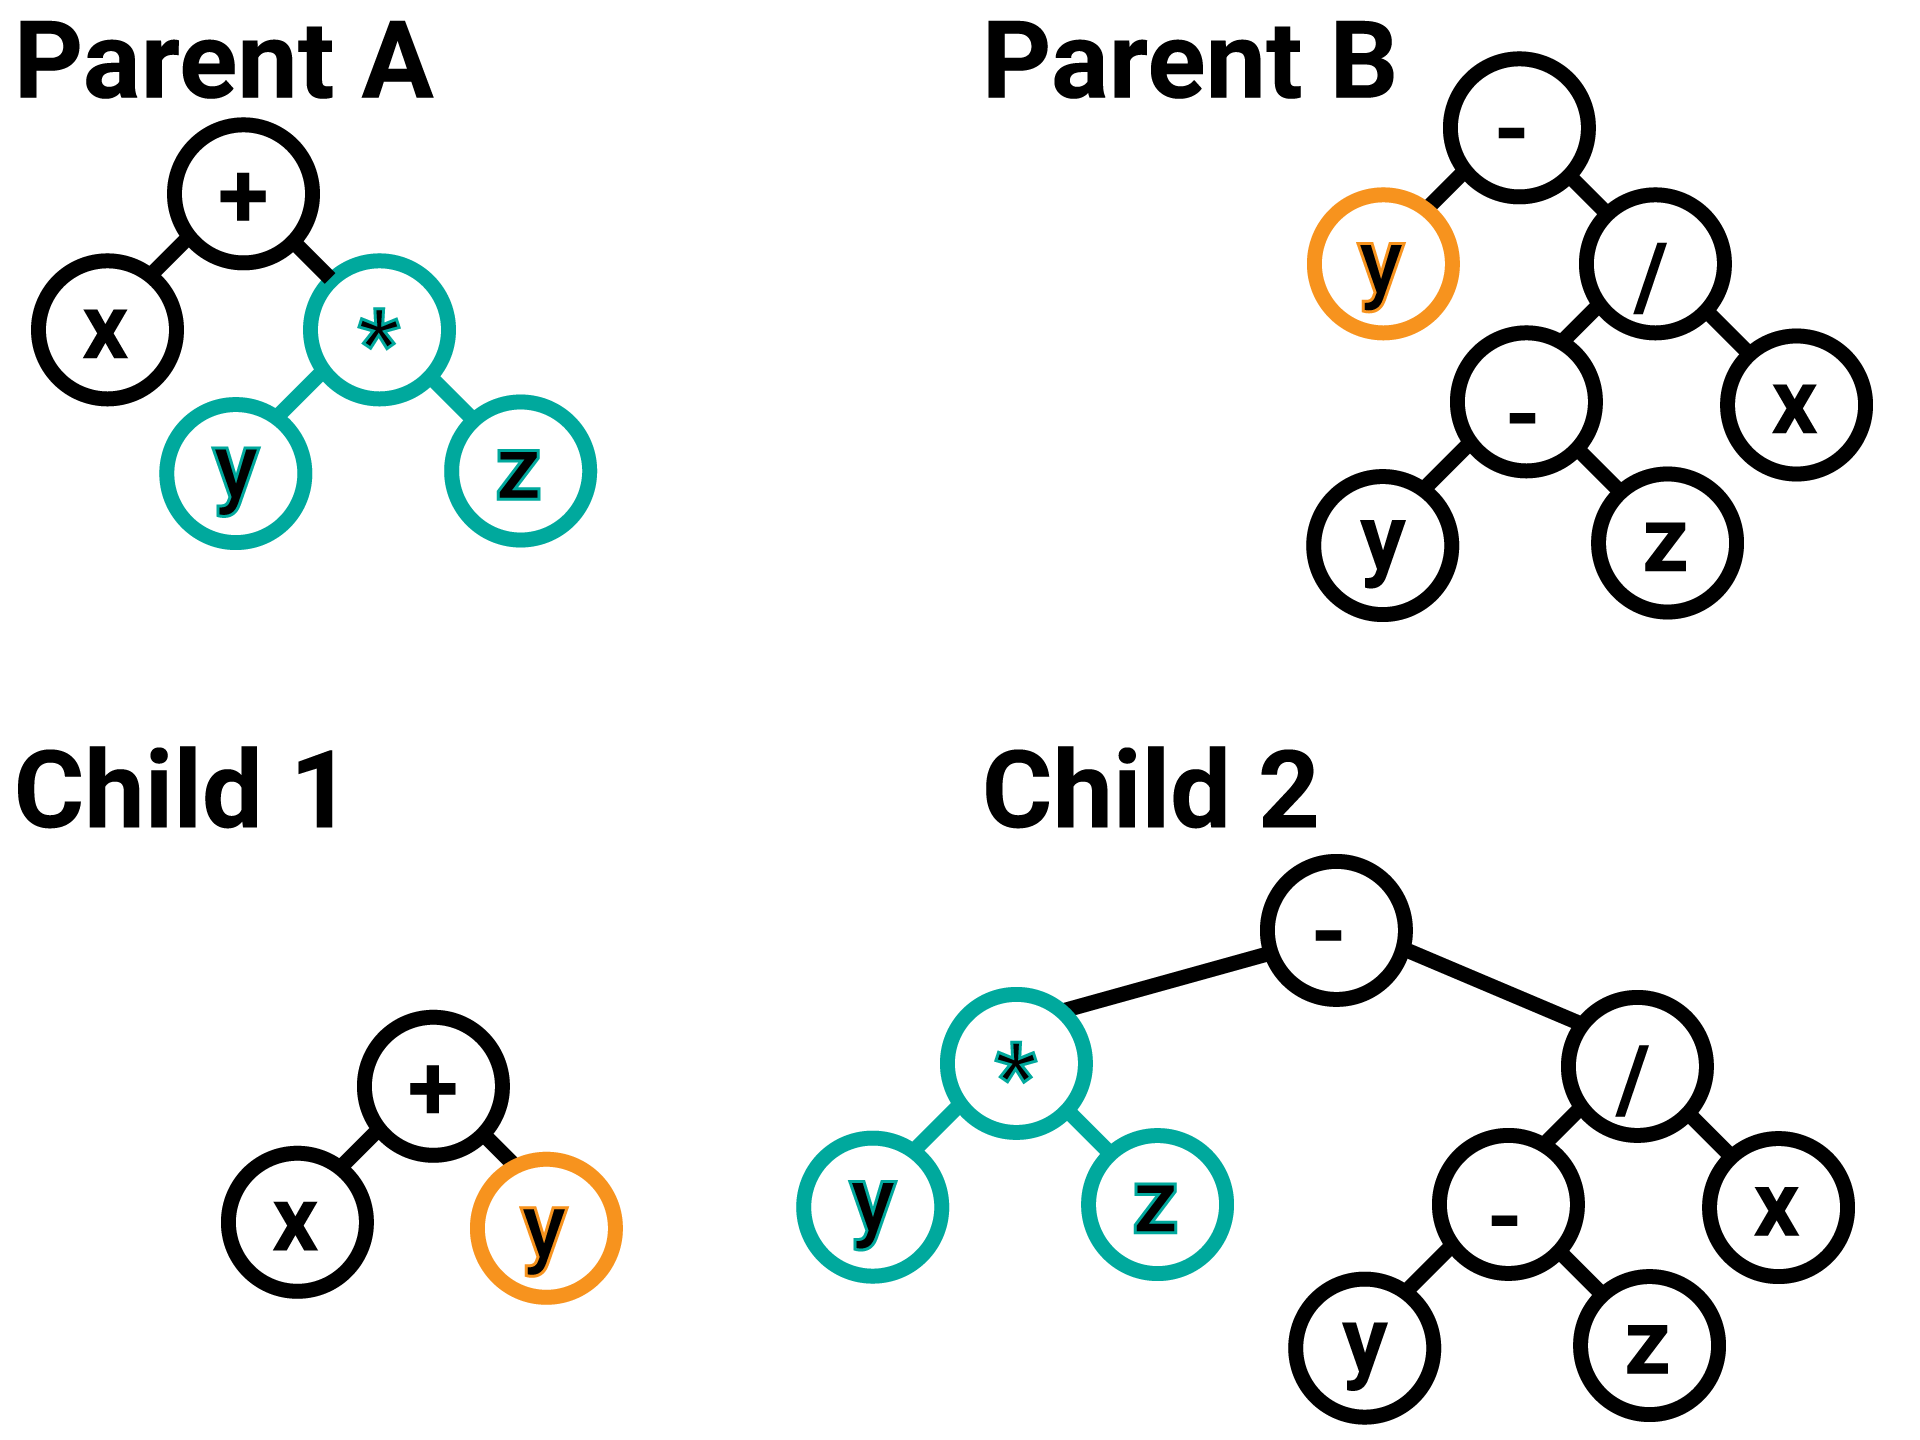
\includegraphics[width=.5\linewidth]{GP}
  \caption{Crossover in GP with two parents producing two offspring}
  \label{fig:GP}
\end{figure}

The evolution process is similar to GAs in that the programs are evaluated using a function which runs a set of test cases and the programs undergo cross-over and other mutations. Cross-over is defined as the exchange of subtrees between programs and produces two offspring from two parents~\cite{Michalewicz1997}, see figure~\ref{fig:GP}.

More advanced versions of GP include function calls which enable the programs to remember useful symmetries and regularities and facilitate code reuse~\cite{Michalewicz1997}.

\subsection{Emerging Evolutionary Algorithms}

This section describes the three algorithms which were benchmarked together with my own algorithm contribution.

\subsubsection{Differential Evolution}

Differential evolution~\cite{Storn1997} is a stochastic optimization algorithm which works on populations of parameter vectors. The problem to minimize will be denoted by $f(x)$ where $X=[x_1,x_2,x_3,...x_D]$ and $D$ is equal to the number of variables taken as input parameters by $f(x)$. The algorithm consists of multiple steps which will be described in detail below. See algorithm~\ref{algo:de}

\begin{algorithm}[h]
  \caption{DE algorithm}
  \label{algo:de}
    \begin{algorithmic}
      \State Initialize population within bounds
      \State Evaluate fitness of population
      \Repeat
        \ForAll{Individuals $x$}
          \State Select three other random individuals a, b and c
          \State Create mutant vector $v=a+F(b-c)$
          \State Create trial vector $u$ by blending $x$ with $v$ (taking at least one gene from $u$)
          \State Replace $x$ with $u$ if $fitness(u) > fitness(x)$
        \EndFor
      \Until{End condition}
    \end{algorithmic}
\end{algorithm}

The first step in DE is to create an initial population, the size of the population is $N$ and it will be represented by a matrix $x$ where $g$ is the generation and $n=1,2,3,...,N$:

\begin{equation}
x_{n,i}^{g} = [ x_{n,1}^{g}, x_{n,2}^{g}, x_{n,3}^{g}, ..., x_{n,D}^{g} ]
\end{equation}

The population is randomly generated to uniformly fill the entire parameter space ($x_{n,i}^U$ is the upper bound for parameter $x_i$ and $x_{n,i}^L$ is the lower bound for parameter $x_i$):

Mutation is the first step when creating a new generation from the population. Mutation is performed individually for every vector $x$ in the population. The mutation procedure is as follows: select three random vectors for each parameter vector (this requires that the population has a size of $N > 3$) and create a set of new vectors $v$ called mutant vectors according to the formula below where $n=1,2,3,...,N$:

\begin{equation}
v_{n}^{g+1} = [ x_{r1n}^{g} + F(x_{r2n}^{g} - x_{r3n}^{g})
\end{equation}

The value of $F$ can be chosen from the interval $[0,2]$ and determines the influence of the differential weight $(x_{r2n}^{g} - x_{r3n}^{g})$.

Crossover occurs after mutation and is applied individually to every vector $x$. A new vector $u$ called the trial vector is constructed from the mutant vector $v$ and the original vector $x$. The trial vector is produced according to the formula below with $i=1,2,3,...,D$ and $n=1,2,3,...,N$:

\begin{equation}
    u_{n,i}^{g+1} =
    \begin{cases}
      v_{n,i}^{g+1}, & \text{if}\ rand() \leq CR \wedge i = I_{\text{rand}} \\
      x_{n,i}^{g}, & \text{otherwise}
\end{cases}
\end{equation}

$I_{\text{rand}}$ is a randomly selected index from the interval $[1,D]$ and $CR$ is the crossover constant which determines the probability that an element is selected from the mutant vector.

Selection is the last step in creating a new generation. The trial vector $u$ is compared with the original vector $x$ for fitness and the vector with the lost cost is selected for the generation according to the formula below where $n=1,2,3,...,N$:

\begin{equation}
    x_{n}^{g+1} =
    \begin{cases}
      u_{n}^{g+1}, & \text{if} f(u_{n}^{g+1}) < f(x_{n}^{g}) \\
      x_{n,i}^{g}, & \text{otherwise}
\end{cases}
\end{equation}

After selection is performed for every vector in the population the population is evaluated to determine if an acceptable solution has been generated. If a solution has been found the algorithm terminates, otherwise the mutation, crossover and selection is performed again until a solution is found or a maximum number of iterations has been reached.

In the benchmark the parameters for DE have been set to $F = 0.6$ and $CR=0.9$ as recommended by Gamperle et al.~\cite{gamperle2002parameter}.

\paragraph{Variants}

Different DE schemes are classified as DE/x/y, where x symbolizes the vector which is mutated and y is the number of differential vectors used. The value of x can be ``rand'' for random vector or ``best''' for the best vector in the population. The algorithm abose is therefore classified as DE/rand/1. The variant DE/best/2 is considered to be a good alternative to DE/rand/1~\cite{qin2009differential}. It's mutation equation is described below:

\begin{equation}
v_{n}^{g+1} = [ x_{best}^{g} + F(x_{r1n}^{g} - x_{r2n}^{g}) + F(x_{r3n}^{g} - x_{r4n}^{g})
\end{equation}

\subsubsection{Particle Swarm Optimization}

Particle Swarm Optimization (PSO)~\cite{Das2008} was introduced in 1995 by Kenneth and Ebenhart~\cite{eberhart1995new}. The optimization problem is represented by an n-dimensional function

\begin{equation}
  f(x_1,x_2,x_3,...x_n) = f(\vec{X})
\end{equation}

where $\vec{X}$ is a vector which represents the real parameters given to the function. The intent is to find a point in the n-dimensional parameter hyperspace that minimizes the function.

PSO is a parallel search technique where a set of particles  fly through the n-dimensional search space and probe solutions along the way. Each particle $P$ has a current position $\vec{x}(t)$, a current velocity $\vec{v}(t)$, a personal best position $\vec{p}(t)$ and the neighborhoods best position $\vec{g}(t)$. A neighborhood $N$ is a collection of particles which act as independent swarms. Neighbourhoods can be social or geographical. Social neighbourhoods do not change and contain the same particles during the entire optimization process, while geographical neighborhoods are dynamic and consist only of particles which are near to one another. The neighborhood is often set to be identical to the whole swarm of particles, denoted $S$.

\begin{figure}[H]
  \centering
  \includegraphics[width=.3\linewidth]{pso}
  \caption{Illustration of particles in PSO}
  \label{fig:pso}
\end{figure}

The algorithm has a set of general properties: $v_{max}$ restricts the velocity of each particle to the interval $[-v_{max},v_{max}]$, an inertial factor $\omega$, two random numbers $\phi_1$ and $\phi_2$ which affect the velocity update formula by modulating the influence of $\vec{p}(t)$ and $\vec{g}(t)$, and two constants $C^2$ and $C^1$ which are termed particle “self-confidence” and “swarm confidence”.

The initial values of $\vec{p}(t)$ and $\vec{g}(t)$ are equal to $\vec{x}(0)$ for each particle. After the particle have been initialized an iterative update process is started which modifies the positions and velocities of the particles. The formula below describes the process ($d$ is the dimension of the position and velocity and $i$ is the index of the particle):

\begin{equation}
  v_{id} (t+1) = \omega v_{id} (t) + C_1 \phi_1 (p_{id} (t) - x_{id} (t)) + C_2 \phi_2 (g_{id} (t) - x_{id} (t))
\end{equation}

\begin{equation}
  x_{id} (t+1) = x_{id} (t) + v_{id} (t+1)
\end{equation}

The “self-confidence” constant affects how much self-exploration a particle is allowed to do while “swarm-confidence” affects how much a particle follows the swarm. $\phi_1$ and $\phi_2$ are random numbers which push the particle in a new direction while $\omega$ keeps a particle on the path it’s currently on. The PSO algorithm is described in algorithm~\ref{algo:pso}. See figure~\ref{fig:pso} for an illustration of PSO.

\begin{algorithm}[h]
  \caption{PSO algorithm}
  \label{algo:pso}
    \begin{algorithmic}
      \State Init particles with random positions
      $\vec{x}(0)$ and velocities $\vec{v}(0)$
      \Repeat
        \ForAll{Particles $i$}
          \State Evaluate fitness $f(\vec{x_i})$
          \State Update $\vec{p}(t)$ and $\vec{g}(t)$
          \State Adapt the velocity of the particle using the above-mentioned equation
          \State Update the position of the particle
        \EndFor
      \Until{$\vec{g}(t)$ is a suitable solution}
    \end{algorithmic}
\end{algorithm}



In the benchmark the parameters for PSO have been set to $\omega = 0.8$~\cite{shi1998modified}, $c_1 = c_2 = 1.494$~\cite{kennedy1999small} and $v_{max} = \text{parameter range size}$~\cite{Das2008}.

\subsubsection{Estimation of Distribution Algorithm}

Estimation of distribution algorithms~\cite{Hauschild2011111} are stochastic search algorithms which try to find the optimal value of a function by creating and sampling probability distributions repeatedly. The first step is creating population $P(0)$ and filling it with solution parameter vectors created from a probability distribution which covers the whole search space uniformly. Then all solutions in $P(g)$ are evaluated and the best solutions $S(g)$ are selected (a threshold variable $t$ is used to determine how many solutions are selected, setting $t=50\%$ means that the best 50\% of the solutions are selected). After selection a probabilistic model $M(g)$ is constructed from $S(g)$ and new solutions $O(g)$ are sampled from $M(g)$. Finally $O(g)$ is incorporated into $P(g)$ The generation counter is incremented $g = g + 1$ and the selection, model and sampling stages are repeated until a suitable solution is found~\cite{Hauschild2011111}.

The most difficult part is constructing the probabilistic model, this will differ for continuous and discreet optimization and a model of appropriate complexity has to be chosen depending on the nature of the problem. The simplest method for continuous EDAs is using a continuous Univariate Marginal Density Algorithm (UMDA). However depending on the complexity of the problem other methods such as Estimation of Baysian Networks (EBNA) can be used~\cite{larranaga2012review}.

\paragraph{UMDA}
The UMDA algorithm is an EDA algorithm which uses a set of independent probability distributions to sample new solution vectors. The probability model can be expressed as a product of the individual probabilities

\begin{equation}
  p(x) = \prod _{d=1}^D {p_d(x_d)}
\end{equation}

where $p(x)$ is the global multivariate density, D is the vector length and $p_d(x_d)$ are the individual univariate marginal densities~\cite{povsik2004estimation}. The algorithm is described in algorithm~\ref{algo:umda}.

\begin{algorithm}[h]
  \caption{UMDA algorithm}
  \label{algo:umda}

    \begin{algorithmic}
      \State Initialize population P with size D
      \Repeat
        \State Evaluate P
        \State Select the best t\% * D individuals from P into S
        \State Let m be the mean of S
        \State Let s be the standard deviation of S
        \State Create a normal distribution ND from m and s
        \State Sample (100\%-t\%) * D individuals into S' from ND
        \State Create new generation of P by combining S' and S
      \Until{Termination condition}
    \end{algorithmic}

\end{algorithm}

\subsection{Machine learning concepts}

The machine learning concepts needed for this thesis are artificial neural networks (ANN), specifically feed-forward neural networks (FFNN). Artificial neural networks are mathematical models which are based on the functioning of biological neurons in the brain. They are useful for predicting future behavior and events, trends, function approximation and data-classification. FFNNs are a popular type of ANN, often referred to as multi-layer perceptrons.  ANNs have to be trained on training data in order to function properly and the most widely used and most popular method for this is back-propagation (BP)~\cite{gardner1998artificial}.

Back-propagation is a local minimization algorithm which works in n-dimensions. It can therefore be replaced by other optimization algorithms such as genetic algorithms. This is what will be considered in the thesis~\cite{gardner1998artificial}.

\subsubsection{Artificial Neuron}

An artificial neuron is a non-linear function with a restricted output range. The unit can take multiple input signals, one threshold signal and produces one output signal. Each input signal has a corresponding weight associated to it which modulates the impact of the input signals by being multiplied with it before entering the unit. The threshold is also represented as a signal with a weight, but the signal's value is always $1$ or $-1$. This means that the threshold signal's weight in fact determines the threshold~\cite{koehn1994combining}. The neuron is illustrated in figure~\ref{figure:artificial_neuron} and equation~\ref{eq:artificial_neuron_math} presents the formula for calculating it's value.

\begin{equation} \label{eq:artificial_neuron_math}
  y = f(-1*w_0+\sum_{i=1}^{n-1}{w_ix_i})
\end{equation}

\begin{figure}[H]
  \centering
    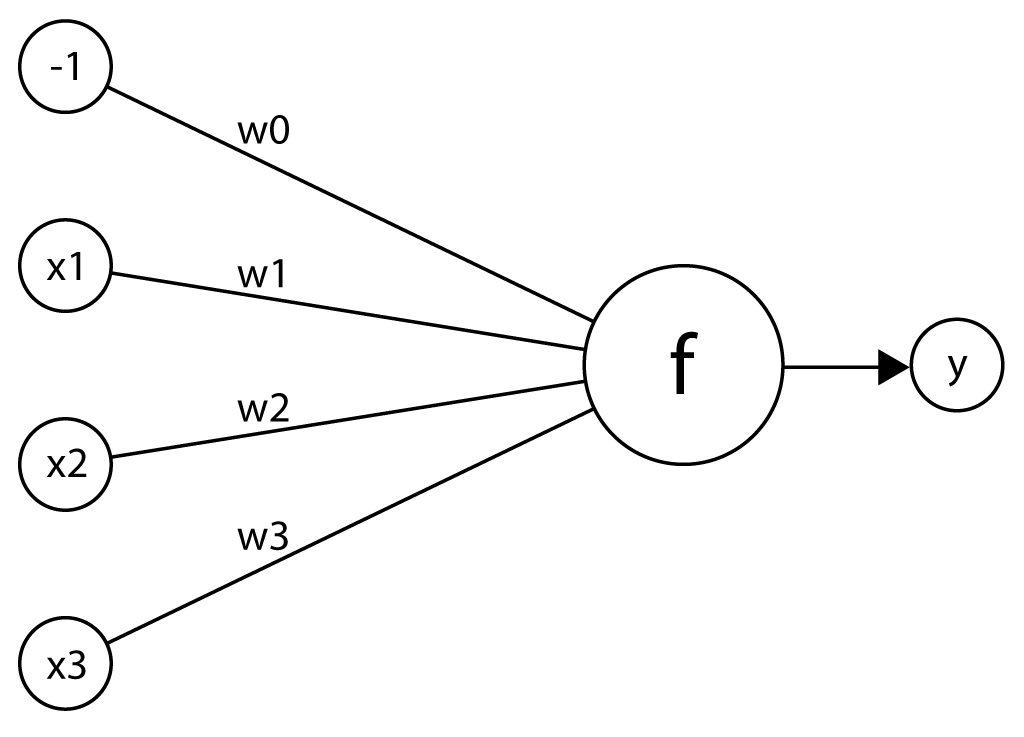
\includegraphics[width=7.5cm]{artificial-neuron}
    \caption{Artificial Neuron}
    \label{figure:artificial_neuron}
\end{figure}

The function $f$ is the so called transfer function, which takes widely ranging input values and maps them to a predetermined output range. The sigmoid function (see equation~\ref{eg:ann_sigmoid_math} and figure~\ref{figure:ann_sigmoid}) is one of the most popular choices for the transfer function because it creates a smooth transition from un-activated to activated neural activity~\cite{koehn1994combining}.

\begin{equation} \label{eg:ann_sigmoid_math}
  \sigma(x)=\frac{1}{1+e^{-x}}
\end{equation}

\begin{figure}[H]
  \centering
    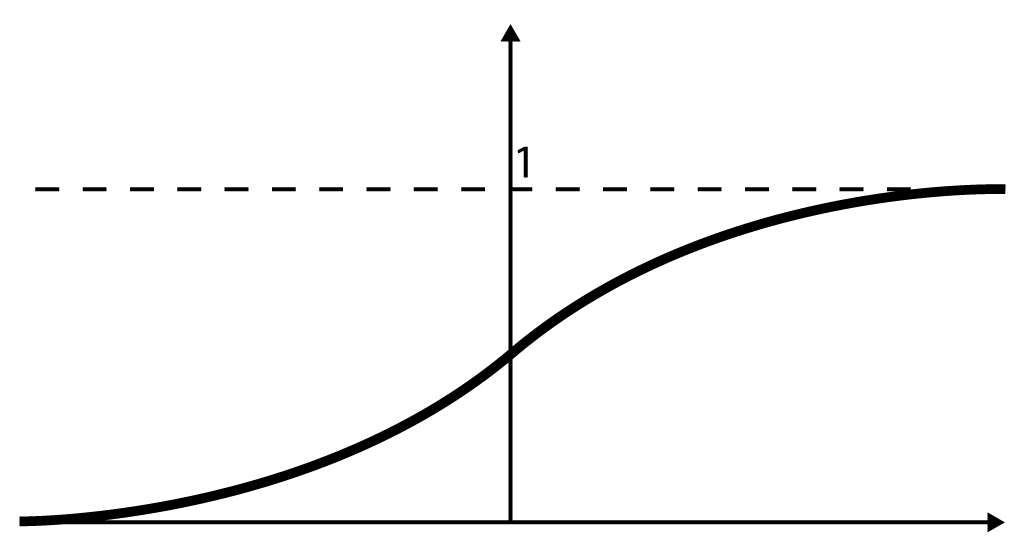
\includegraphics[width=7.5cm]{sigmoid}
    \caption{Sigmoid function}
    \label{figure:ann_sigmoid}
\end{figure}

\subsubsection{Artificial Neural Networks}
Artificial Neural Networks(ANN) consists of multiple neurons grouped together. In the widely used version called Feed-Forward Neural Network(FFNN)~\cite{montana1989training} the network is grouped into three basic layers:
\begin{enumerate}
  \item An input layer, which takes a vector of inputs
  \item One or more hidden layers, which process the data
  \item An output layer, which produces usable output data
\end{enumerate}
Neurons in FFNNs are always connected to all neurons in the preceding and succeeding layers and the connection form no closed loops~\cite{yao1999evolving}. Figure~\ref{figure:FFNN} shows a simple network with two neurons ($z_1$ and $z_2$) in the input layer, which are linked to three hidden neurons ($y_1$, $y_2$ and $y_3$), which are in turn linked to two output neurons ($o_1$ and $o_2$). The weights are represented by $v_{ij}$ and $w_{ij}$.

\begin{figure}[H]
  \centering
    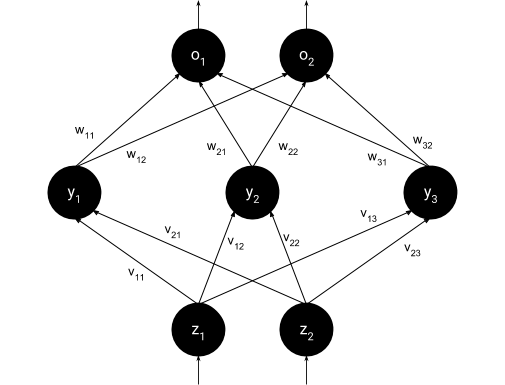
\includegraphics[width=10cm]{FFNN}
    \caption{Feed-Forward Neural Network}
    \label{figure:FFNN}
\end{figure}

The FFNN is evaluated by evaluating the individual neurons in each layers beginning from the input layer and moving successively forward until the output layer is reached. The values calculated at the output neurons is treated as the output from the network.

\subsubsection{Back-propagation}

Back-propagation~\cite{koehn1994combining} is a neural network training algorithm which uses sets of training data to teach a neural network different patterns. The training data consists of a set inputs and corresponding outputs. Initially the network will have random weights and the network will not yield the correct output for most of the training inputs. Back-propagation works by slightly adjusting the weights for each training sample. This is done repeatedly and once cycle through all training samples is referred to as an epoch.

The gradient descent algorithms is used to accomplish this by optimizing the error function of the network (see equation~\ref{eg:bp_error}) which is the sum of squared errors, the error being the difference between the actual network outputs ($o_k$) and the correct training outputs($t_k$).

\begin{equation} \label{eg:bp_error}
  E=\frac{1}{2}\sum_{k\in outputs}^{}{(t_k-o_k)^2}
\end{equation}

The equations for updating the weights~\cite{koehn1994combining} are dependent on the transfer function's derivative. Equation~\ref{eg:sigmoid_d} shows the sigmoids derivative which is basis for the weight update formulae in equations~\ref{eg:w_update1},~\ref{eg:w_update2} and~\ref{eg:w_update3}.

\begin{equation} \label{eg:sigmoid_d}
  \frac{d}{dx}\sigma(x)=\sigma(x)(1-\sigma(x))
\end{equation}

\begin{equation} \label{eg:w_update1}
  \Delta w_{from,to} = -\lambda o_{from}\delta_{to}
\end{equation}

\begin{equation} \label{eg:w_update2}
  \delta_{output} = (t_{output}-o_{output})o_{output}(1-o_{output})
\end{equation}

\begin{equation} \label{eg:w_update3}
  \delta_{hidden} = -(1-o_{hidden})o_{hidden} \sum_{i}^{}{\delta_{i}w_{hidden,i}}
\end{equation}
